\documentclass[presentation,professionalfonts]{beamer}


\usepackage[utf8]{inputenc}
\usepackage[T1]{fontenc}
\usepackage{graphicx}
\usepackage[normalem]{ulem}
\usepackage{amsmath}
\usepackage{IEEEtrantools}
\usepackage{bm}
\usepackage{hyperref}
\tolerance=1000
\usepackage{algorithm}
\usepackage{algpseudocode}
\usepackage{tikz}
\usepackage{xspace}
\usepackage{booktabs}
\usepackage{listings}
\usepackage{appendixnumberbeamer}

\usepackage[
backend=biber,
style=numeric,
sortlocale=en_US,
url=false,
doi=true,
eprint=false,
giveninits=false,
maxbibnames=20,
maxnames=20,
maxcitenames=4
]{biblatex}
\addbibresource{templ.bib}

\usepackage{lmodern}
\usefonttheme[onlymath]{serif}

\setbeamercovered{highly dynamic}
\setbeamertemplate{caption}[numbered]
\setbeamertemplate{bibliography item}[text]
\usetheme{TUW}

\newcommand{\semname}{Scheduling Algorithms for Clusters, Distributed Systems, and Multi-core Nodes}
\newcommand{\semester}{SS 2018}

\institute[TU Wien]{Seminar ``\semname''\\\semester}
\titlegraphic{
\includegraphics[height=.7cm]{./logos/par-logo.pdf}\quad
\includegraphics[height=.7cm]{./logos/info-logo.pdf}}

% change this, of course
\date{\today}
\title[Scheduling Jobs with Max-Min Fairness]{Scheduling Jobs across Geo-Distributed Datacenters with Max-Min Fairness}
\author[Aleksandr Lisianoi]{Aleksandr Lisianoi}

\begin{document}

\maketitle

\begin{frame}{Seminar Talk's Main Sources}
  \begin{enumerate}
  \item \fullcite{Chen2017}
  \item \fullcite{Meyer1976}
  \end{enumerate}
\end{frame}

\AtBeginSection[]
{
 \begin{frame}<beamer>
 \frametitle{Plan}
 \tableofcontents[currentsection]
 \end{frame}
}

%% \begin{frame}{Outline}
%%   % \tableofcontents[currentsection]
%%   \tableofcontents
%% \end{frame}

\section{Introduction}

\begin{frame}{Problem Description}
    Given a \emph{large amount} of data distributed across
    \emph{geographically separate} datacenters, how to efficiently run
    \emph{multiple analytic jobs} in a \emph{fair} fashion?
\end{frame}

\begin{frame}{Typical Analytic Jobs}
  \begin{itemize}
  \item 2007 The New York Times: ~4 TiB, <24 hours \\
    (\href{https://open.blogs.nytimes.com/2007/11/01/self-service-prorated-super-computing-fun/}{online article}, last access 21.04.2018)
  \item 2017 ALS at Spotify: ~100 PiB, ~2500 nodes, ~20k jobs per day \\
    (\href{https://labs.spotify.com/2017/10/16/big-data-processing-at-spotify-the-road-to-scio-part-1/}{online article}, last access 21.04.2018)
  \end{itemize}
\end{frame}

\begin{frame}{Large Amounts of Data and Geography}
  \begin{itemize}
  \item Data locality
  \item Network speed
  \end{itemize}
\end{frame}

\begin{frame}{Fairness}
  \emph{Fairness}: all the participants get a fair share of the
  resources.
  \\~\\
  \emph{Max-Min fairness}: any attempt to increase any participant's
  share decreases some non-larger share of another participant.
\end{frame}

\section{Model and Formulation}

\begin{frame}{Background Definitions}
  \begin{IEEEeqnarray*}{llCl}
    \text{Datacenter: }                 & \mathcal{D}   &=& \left\{1, 2, \dots, J\right\} \\
    \text{Datacenter capacity: }        & \mathcal{A}   &=& \left\{a_1, a_2, \dots, a_J\right\} \\
    \text{Analytic job: }               & \mathcal{K}   &=& \left\{1, 2, \dots, K\right\} \\
    \text{Parallel tasks of a job: }    & \mathcal{T}_k &=& \left\{1, 2, \dots, n_k\right\} \\
    \text{Execution time of a task: }                 & e^k_{i, j} \\
    \text{Network transfer time of a task: } & c^k_{i, j}
  \end{IEEEeqnarray*}
\end{frame}

\newcommand{\flvr}{\langle\bm{v}\rangle}
\newcommand{\fbma}{\bm{\alpha}}
\newcommand{\flar}{\langle\fbma\rangle}
\newcommand{\fbmb}{\bm{\beta}}
\newcommand{\flbr}{\langle\fbmb\rangle}

\begin{frame}{Lexicographic Minimization}
  \begin{definition}[Non-increasingly sorted \(\langle\bm{v}\rangle\)]
    Let \(\flvr_k\) denote the \(k\)-th (\(1\leq k \leq K\)) largest element of \(\bm{v}\in\mathbb{Z}^K\), implying \(\flvr_1\geq\flvr_2\dots\geq\flvr_K\). Then \(\bm{\flvr} = \left(\flvr_1, \flvr_2, \dots, \flvr_K\right)\) represents the non-increasingly sorted version of \(\bm{v}\).
  \end{definition}
  \begin{definition}[Lexicographically smaller vector]
    For any \(\fbma\in\mathbb{Z}^K, \fbmb\in\mathbb{Z}^K\), if \(\flar_1\leq\flbr_1\) or \(\exists k\in \left\{1,2,\dots, K\right\}\) s.t. \(\flar_k\leq\flbr_k\) and \(\flar_i = \flbr_i, \forall i\in [1, \dots, k)\), then \(\fbma\) is lexicographically smaller than \(\fbmb\), denoted \(\fbma \preceq \fbmb\).
  \end{definition}
  \begin{definition}[Lexicographic minimization]
    Lexicographic minimization of vector \(\bm{f}\) is represented with \(\text{lexmin}_{\bm{x}}\bm{f}\) with the optimal solution \(\bm{x^*}\in\mathbb{R}^K\) s.t. \(\forall \bm{x}\in\mathbb{R}^K: \bm{f}(\bm{x^*})\preceq\bm{f}(\bm{x})\)
    \end{definition}
  \end{frame}

\newcommand{\foralltdk}{\forall i \in \mathcal{T}_k, \forall j\in\mathcal{D}, \forall k\in\mathcal{K}}
\newcommand{\fcapacity}{\sum_{k\in\mathcal{K}}\sum_{i\in\mathcal{T}_k} x^k_{i, j} \leq a_j}
\newcommand{\fcapacityq}{\forall j\in\mathcal{D}}
\newcommand{\fpresence}{\sum_{j\in\mathcal{D}}x^k_{i, j} = 1}
\newcommand{\fpresenceq}{\forall i\in\mathcal{T}_k, \forall k\in\mathcal{K}}

\begin{frame}{First Optimization Problem}
  \begin{IEEEeqnarray}{lrCll}
    \text{lexmin}_{\bm{x}} & \bm{f} &=&\left(\tau_1, \tau_2, \dots, \tau_K\right) &\\
    \text{s.t.} & \tau_k &=& \max_{i\in\mathcal{T}_k, j\in\mathcal{D}} x^k_{i, j}\left(c^k_{i, j} + e^k_{i, j}\right), &\forall k\in\mathcal{K} \label{eq:goal}\\
    &&& \fcapacity,  &\fcapacityq\label{eq:capacity}\\
    &&& \fpresence,  &\fpresenceq\label{eq:presence}\\
    &&& x^k_{i, j} \in \left\{0, 1\right\}. &\foralltdk\label{eq:onehot}
  \end{IEEEeqnarray}

  Constraint \eqref{eq:goal}: a job requires as long as its longest task. \\
  Constraint \eqref{eq:capacity}: capacity of the datacenter is not exceeded. \\
  Constraint \eqref{eq:presence}: each task is assigned to exactly one datacenter. \\
\end{frame}

\begin{frame}{Transformation Plan}
  \begin{itemize}
  \item Separable convex objective:
    \begin{IEEEeqnarray*}{rCl}
      f(x_1, x_2, \dots, x_K) &=& \sum_{i=1}^K f_i(x_i) \\
      f(\alpha_1 x_1 + \alpha_2 x_2) &\leq& \alpha_1 f(x_1) + \alpha_2 f(x_2), \text{ where } \\
      \alpha_1 + \alpha_2 &=& 1
    \end{IEEEeqnarray*}
  \item Totally unimodular linear constraints:
    matrix \(M\) is a \emph{totally unimodular matrix} if its
    every \emph{square submatrix} \(A\) has \(\det A\in \{-1, 0,
    1\}\)
  \end{itemize}

  Then apply \(\lambda\)-representation technique to compute solution \cite{Meyer1976}.
\end{frame}

\begin{frame}{Towards Single Objective and Linear Constraints}
  From multiple-objective to single-objective optimization:
  \begin{IEEEeqnarray}{ll}
    \min_{\bm{x}} & \quad \max_{k\in\mathcal{K}}\left(\tau_k\right) \\
    \text{s.t.}  & \quad \text{Constraints \eqref{eq:goal}, \eqref{eq:capacity}, \eqref{eq:presence} and \eqref{eq:onehot} hold}
  \end{IEEEeqnarray}

  \pause

  From non-linear constraints to linear constraints:

  \begin{IEEEeqnarray}{ll}
    \min_{\bm{x}} & \quad \max_{k\in\mathcal{K}}\left(\max_{i\in\mathcal{T}_k, j\in\mathcal{D}} x^k_{i, j}\left(c^k_{i, j} + e^k_{i, j}\right)\right) \\
    \text{s.t.}  & \quad \text{Constraints \eqref{eq:capacity}, \eqref{eq:presence} and \eqref{eq:onehot} hold}
  \end{IEEEeqnarray}

  \pause

  \begin{equation*}
        \text{Define: }\phi (x^k_{i, j}) = x^k_{i, j} (c^k_{i, j} + e^k_{i, j}), \forall i\in\mathcal{T}_k, j\in \mathcal{D}, k\in\mathcal{K}
  \end{equation*}

  \pause

  From minimizing the triple maximum to lexicographic minimization:
  \begin{IEEEeqnarray}{ll}
    \text{lexmin}_{\bm{x}} & \quad \bm{g} = \left(\phi(x^1_{1, 1}), \dots, \phi(x^k_{i, j}), \dots, \phi(x^K_{n_k, J})\right) \\
    \text{s.t.}           & \quad \text{Constraints \eqref{eq:capacity}, \eqref{eq:presence} and \eqref{eq:onehot} hold}
  \end{IEEEeqnarray}
\end{frame}

\begin{frame}{Towards a Separable Objective Function}
  \begin{IEEEeqnarray*}{lCl}
    \text{Define: }g^m &=& \text{element of vector }\bm{g}\text{ at position }m \\
    \text{Define: }M &=& |\bm{g}| = J\sum_{k = 1}^{K}n_k \\
    \text{Define: }\varphi(\bm{g}) &=& \sum_{m = 1}^{M}M^{g_m}
  \end{IEEEeqnarray*}
  \begin{lemma}
    \(\varphi(.)\) preserves the order of ``lexicographically no greater'' \(\preceq\), i.e.
    \[\bm{g}(x^*) \preceq \bm{g}(x) \iff \varphi(\bm{g}(x^*)) \leq\varphi(\bm{g}(x))\]
  \end{lemma}
\end{frame}

\begin{frame}{Transformation Plan Complete}
  \newcounter{x}\setcounter{x}{\value{equation}}\setcounter{equation}{5}
  \begin{IEEEeqnarray}{lrCll}
    \min_{\bm{x}} &&& \max_{k\in\mathcal{K}}\left(\tau_k\right) \\
    \setcounter{equation}{2}
    \text{s.t.} & \tau_k &=& \max_{i\in\mathcal{T}_k, j\in\mathcal{D}} x^k_{i, j}\left(c^k_{i, j} + e^k_{i, j}\right), &\forall k\in\mathcal{K} \\
    &&& \fcapacity,  &\fcapacityq \\
    &&& \fpresence,  &\fpresenceq \\
    &&& x^k_{i, j} \in \left\{0, 1\right\}. &\foralltdk
  \end{IEEEeqnarray}
  \setcounter{equation}{\value{x}}

  \begin{IEEEeqnarray}{ll}
    \min_{\bm{x}} & \quad \sum_{k\in\mathcal{K}}\sum_{i\in\mathcal{T}_k}\sum_{j\in\mathcal{D}} M^{\varphi(x^k_{i, j})} \\
    \text{s.t.}  & \quad \text{Constraints \eqref{eq:capacity}, \eqref{eq:presence} and \eqref{eq:onehot} hold}
  \end{IEEEeqnarray}
\end{frame}

\newcommand{\flambdas}{\lambda^{k, 0}_{i, j} + \lambda^{k, 1}_{i, j}}
\newcommand{\fsmember}{\flambdas M^{\left(c^k_{i, j} + e^k_{i, j}\right)}}
\newcommand{\rplus}{\mathbf{R}^{+}}

\begin{frame}{Towards Removing Integrality Constraints}
  Lambda representation technique:
  \begin{IEEEeqnarray}{lCl}
    M^{\varphi\left(x^k_{i, j}\right)} &=& \sum_{s\in\{0,1\}} \lambda^{k, s}_{i, j}M^{s\left(c^k_{i, j} + e^k_{i, j}\right)} = \fsmember \IEEEeqnarraynumspace\\
    x^k_{i, j} &=& \sum_{s\in\{0, 1\}}s\lambda^{k, s}_{i, j} = \lambda^{k, 1}_{i, j} \\
    \sum_{s\in\{0, 1\}} \lambda^{k, s}_{i, j} &=& \flambdas = 1 \\
    \lambda^{k, s}_{i, j} &\in& \rplus
    \end{IEEEeqnarray}
\end{frame}

\begin{frame}{Integrality Constraints Removed}
  \begin{IEEEeqnarray}{Cl}
    \min_{\bm{x}, \bm{\lambda}} & \quad \sum_{k\in\mathcal{K}}\sum_{i\in\mathcal{T}_k}\sum_{j\in\mathcal{D}} \left(\fsmember\right) \\
    \text{s.t.}  & \quad x^k_{i, j} = \lambda^{k, 1}_{i, j}, \foralltdk \\
                 & \quad \flambdas = 1, \foralltdk \\
                 & \quad x^k_{i, j}, \lambda^{k, 0}_{i, j}, \lambda^{k, 1}_{i, j} \in \rplus, \foralltdk \\
    & \quad \fcapacity, \fcapacityq \\
    & \quad \fpresence, \fpresenceq
  \end{IEEEeqnarray}
\end{frame}

\begin{frame}{Back to Multiobjective Optimization}
  Subproblem produces \((k^*, i^*, j^*)\) with longest completion time
  \\~\\
  Set \(x^{k^*}_{i^*, j^*} = 1\) and \(x^{k^*}_{i^*, j} = 0, j\neq j^*\), remove from \(\bm{x}\)
  \\~\\
  Set completion times for \(x^{k^*}_{i, j}\), where \((i, j)\neq
  (i^*, j^*)\), to the worst completion time
  \end{frame}

\section{Experimental Evaluation}

\begin{frame}{Architecture}
  \begin{itemize}
  \item Describe computation job as a DAG of tasks, submit to DAG scheduler
  \item DAG scheduler divides DAG of tasks into stages, iteratively submits each stage to task scheduler
  \item Task scheduler reimplemented to solve the optimization problem
  \item Example problem is legacy \texttt{Sort}, 3 tasks per job, each
    task starts with 100 MiB of data in its datacenter. Measured
    groups of 3, 4 and 5 concurrent jobs
  \end{itemize}
  \end{frame}

\begin{frame}{Execution}
  \begin{itemize}
  \item Across 6 datacenters of Amazon EC2 spin up 2 \texttt{m3.large} VMs in each
  \item Ubuntu Server 14.04 LTS, Spark 1.6.1, Hadoop 2.6.4, Java 1.8, Scala 2.11.8
  \item Spark cluster in standalone mode, no external resource manager (e.g. YARN)
  \end{itemize}
\end{frame}

\begin{frame}
  \frametitle{Experimental Results}
  \begin{center}
  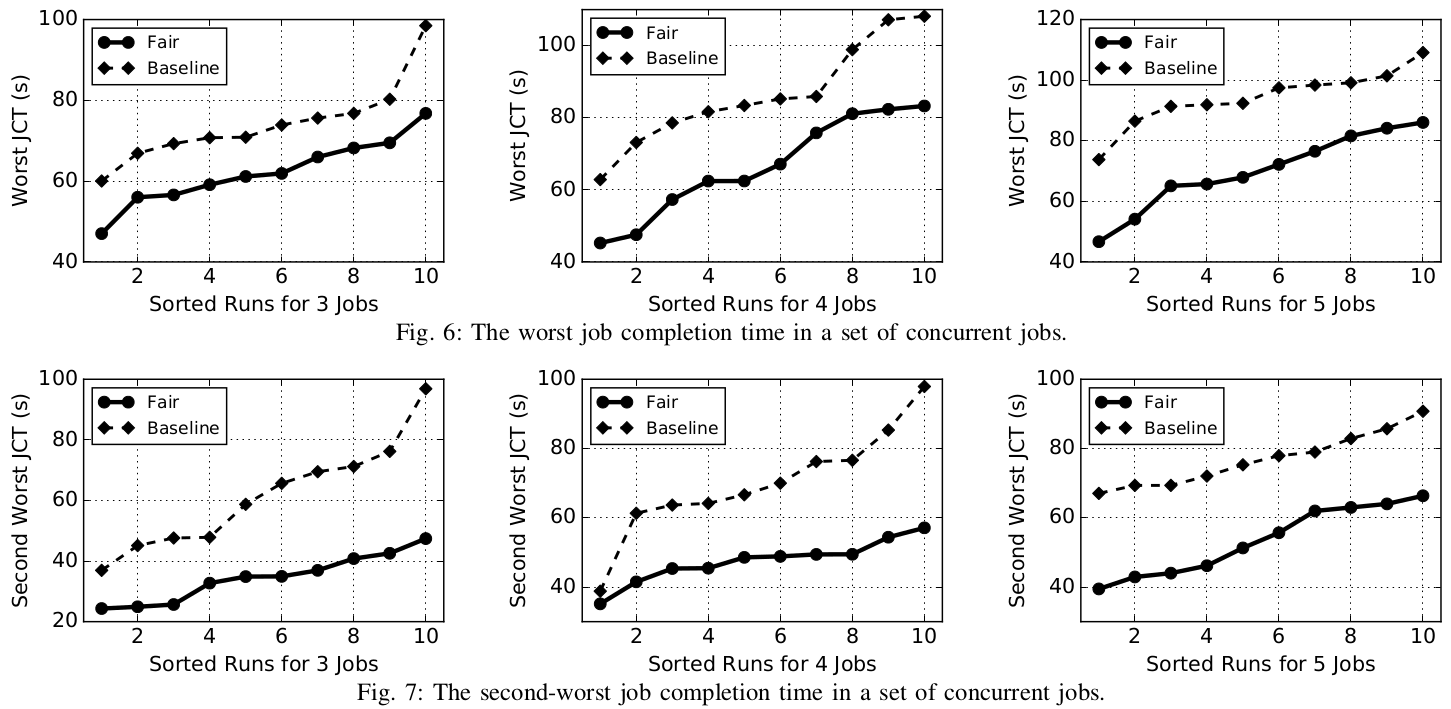
\includegraphics[width=\textwidth]{main_result}\\
  image source: \textcite{Chen2017}
  \end{center}
\end{frame}

\section{Conclusions}

\begin{frame}
  \frametitle{Conclusions}
  \begin{itemize}
  \item Reproducibility problems:
    \begin{itemize}
    \item No source code
    \item Could not find legacy \texttt{Sort} application
    \end{itemize}
  \item Not clear how the 4 and 5 job variants differ:
  \item Convincingly outperformed default Spark scheduler
  \end{itemize}
\end{frame}


\begin{frame}[fragile]{References}
\printbibliography
\end{frame}

\appendix

\begin{frame}{Unimodular Matrix}
  \begin{definition}[Unimodular Matrix]
    Matrix \(M\) is a \emph{unimodular matrix} if it is a \emph{square}, \emph{integer} matrix with \[\det M = \pm 1\]
  \end{definition}
  \begin{definition}[Unimodular Matrix]
    Matrix \(M\) is a \emph{unimodular matrix} if it is an
    \emph{integer}, \emph{invertible} matrix and its inverse is also
    an \emph{integer}, \emph{invertible} matrix.
  \end{definition}
  Examples: identity matrix, \emph{permutation matrix}, pascal matrix, \dots
\end{frame}

\begin{frame}{Totally Unimodular Matrix}
  \begin{definition}{Totally Unimodular Matrix}
    Matrix \(M\) is a \emph{totally unimodular matrix} if its every
    non-singular square submatrix is unimodular.
  \end{definition}

  \begin{definition}{Totally Unimodular Matrix}
    Matrix \(M\) is a \emph{totally unimodular matrix} if its every
    \emph{square submatrix} \(A\) has \(\det A\in \{-1, 0, 1\}\)
  \end{definition}

  \begin{definition}{Totally Unimodular Matrix}
    Matrix \(A\) is a \emph{totally unimodular matrix} if its every
    element \(A_{i, j}\in \{-1, 0, 1\}\) and any row subset \(R\) can
    be divided into two disjoint subsets \(R_1\) and \(R_2\) s.t.
    \[\left|\sum_{i\in R_1} a_{i, j} - \sum_{i\in R_2}a_{i, j}\right| \leq 1, \forall j\in{1, 2, \dots, n}\]
    \end{definition}
\end{frame}

\begin{frame}{Totally Unimodular Matrices in Optimization}
  Important well-known optimization fact: if \(M\) is totally
  unimodular and \(b\) is integral, then linear programs \(\left\{\min
  cx | Mx \geq b, x\geq 0\right\}\) and \(\{\max cx | Mx \leq b\}\)
  have integral optima for any \(c\).
\end{frame}

\end{document}
